% SOURCE-MATCHED VERSION: 2026-08-23 12:18 +07
% This exact file is the source used to compile lecture3_bigO_SOURCE_MATCHED_20260823.pdf
\documentclass[aspectratio=169]{beamer}

\usepackage[utf8]{inputenc}
\usepackage[english]{babel}
\usepackage{booktabs}
\usepackage{array}
\usepackage{graphicx}
\usepackage{listings}
\usepackage{tikz}
\usetikzlibrary{arrows.meta,positioning,shapes.geometric}


\usepackage{empheq}
\usepackage{tcolorbox}
\tcbuselibrary{skins,theorems}

\newtcbox{\mymath}[1][]{%
    nobeforeafter, math upper, tcbox raise base,
    enhanced, colframe=blue!30!black,
    colback=blue!30, boxrule=1pt,
    #1}



\graphicspath{{images/}{figures/}{logo/}{../logo/}}

\definecolor{ForestGreen}{RGB}{22,100,70}
\definecolor{SoftGreen}{RGB}{229,244,235}
\definecolor{SoftBlue}{RGB}{226,239,255}
\definecolor{SoftOrange}{RGB}{255,241,220}
\definecolor{SoftPurple}{RGB}{239,231,255}

\newcolumntype{L}[1]{>{\raggedright\arraybackslash}p{#1}}

\mode<presentation>{
  \usetheme{Ilmenau}
  \usecolortheme{spruce}
  \usefonttheme{professionalfonts}
  \setbeamertemplate{navigation symbols}{}
  \setbeamertemplate{headline}{}
  \setbeamertemplate{caption}[numbered]
  \setbeamercolor{institute in head/foot}{fg=ForestGreen}
}

\lstset{
  language=Python,
  basicstyle=\ttfamily\footnotesize,
  keywordstyle=\color{blue!75!black}\bfseries,
  stringstyle=\color{red!65!black},
  commentstyle=\color{ForestGreen},
  numbers=left,
  numberstyle=\tiny\color{gray},
  numbersep=6pt,
  showstringspaces=false,
  keepspaces=true,
  columns=fullflexible,
  breaklines=true,
  frame=single,
  rulecolor=\color{ForestGreen!60},
  backgroundcolor=\color{SoftGreen!35},
  tabsize=4
}

\lstdefinestyle{pseudo}{
  basicstyle=\ttfamily\scriptsize,
  keywordstyle=\color{blue!75!black}\bfseries,
  morekeywords={ALGORITHM,FUNCTION,PROCEDURE,INPUT,OUTPUT,IF,THEN,ELSE,
    ELSEIF,RETURN,FOR,EACH,IN,TO,DO,WHILE,REPEAT,UNTIL,END,MOD,DIV,
    CREATE,SET,REMOVE,INFINITY,NONE,TRUE,FALSE,SQRT,LENGTH},
  numbers=none,
  showstringspaces=false,
  keepspaces=true,
  columns=fullflexible,
  breaklines=true,
  frame=single,
  rulecolor=\color{ForestGreen!60},
  backgroundcolor=\color{SoftBlue!35},
  tabsize=4
}

\lstdefinestyle{pseudonumbered}{
  basicstyle=\ttfamily\scriptsize,
  keywordstyle=\color{blue!75!black}\bfseries,
  morekeywords={ALGORITHM,FUNCTION,PROCEDURE,INPUT,OUTPUT,IF,THEN,ELSE,
    ELSEIF,RETURN,FOR,EACH,IN,TO,DO,WHILE,REPEAT,UNTIL,END,MOD,DIV,
    CREATE,SET,REMOVE,INFINITY,NONE,TRUE,FALSE,SQRT,LENGTH},
  numbers=left,
  numberstyle=\tiny\color{gray},
  numbersep=6pt,
  showstringspaces=false,
  keepspaces=true,
  columns=fullflexible,
  breaklines=true,
  frame=single,
  rulecolor=\color{ForestGreen!60},
  backgroundcolor=\color{SoftBlue!35},
  tabsize=4
}

\tikzset{
  concept/.style={draw=ForestGreen,rounded corners,fill=SoftGreen,
    very thick,minimum height=1.05cm,text width=3.1cm,align=center},
  process/.style={draw=blue!60!black,rounded corners,fill=SoftBlue,
    thick,minimum height=0.95cm,text width=2.7cm,align=center},
  decision/.style={diamond,draw=orange!75!black,fill=SoftOrange,
    thick,aspect=2.1,text width=2.1cm,align=center,inner sep=1pt},
  data/.style={trapezium,trapezium left angle=70,trapezium right angle=110,
    draw=purple!65!black,fill=SoftPurple,thick,minimum height=0.9cm,
    text width=2.4cm,align=center},
  smallbox/.style={draw=ForestGreen,rounded corners,fill=SoftGreen,
    thick,minimum height=0.85cm,text width=2.2cm,align=center,font=\small},
  arrow/.style={-Latex,very thick,ForestGreen}
}

\newcommand{\TitleLogo}{%
  \IfFileExists{logo/logo_slide.png}{\includegraphics[width=0.27\textwidth]{logo/logo_slide.png}}{%
  \IfFileExists{../logo/logo_slide.png}{\includegraphics[width=0.27\textwidth]{../logo/logo_slide.png}}{%
  \IfFileExists{logo_slide.png}{\includegraphics[width=0.27\textwidth]{logo_slide.png}}{%
  \fcolorbox{ForestGreen}{ForestGreen}{\parbox[c][0.85cm][c]{0.27\textwidth}{\centering\color{white}\bfseries NEU -- DS\&AI}}}}}%
}
\newcommand{\FooterLogo}{%
  \IfFileExists{logo/logo_fda.png}{\includegraphics[width=0.8cm]{logo/logo_fda.png}}{%
  \IfFileExists{../logo/logo_fda.png}{\includegraphics[width=0.8cm]{../logo/logo_fda.png}}{%
  \IfFileExists{logo_fda.png}{\includegraphics[width=0.8cm]{logo_fda.png}}{%
  \fcolorbox{ForestGreen}{ForestGreen}{\parbox[c][0.45cm][c]{0.8cm}{\centering\color{white}\scriptsize FDA}}}}}%
}

\title[DSAI1002 - Part 03]{Data Structures and Algorithms in Python\\Lecture 4: Asymptotic Analysis and Big-O Notation}
\author{Faculty of Data Science and Artificial Intelligence}
\institute{National Economics University}
\date{}

\AtBeginSection[]{
  \begin{frame}[plain]
    \begin{center}
      \vfill
      {\color{ForestGreen}\large\bfseries SECTION \insertsectionnumber}
      \vspace{0.8em}
      {\color{ForestGreen}\rule{0.68\textwidth}{1.2pt}}
      \vspace{1.1em}
      {\usebeamerfont{section title}\color{ForestGreen}\Huge\bfseries
        \insertsectionhead}
      \vspace{1.1em}
      {\color{ForestGreen}\rule{0.68\textwidth}{1.2pt}}
      \vfill
    \end{center}
  \end{frame}
}

\begin{document}

\begin{frame}[plain]
  \setbeamercolor{block body example}{bg=ForestGreen,fg=white}
  \begin{center}
    \begin{beamercolorbox}[wd=\textwidth,sep=1pt,center,rounded=true,shadow=true]{block body example}
      \TitleLogo
    \end{beamercolorbox}
  \end{center}
  \vspace{-0.25em}
  \titlepage
\end{frame}

\logo{\FooterLogo}
\setbeamertemplate{footline}{%
  \begin{beamercolorbox}[colsep=1.5pt]{upper separation line foot}
  \end{beamercolorbox}
  \begin{beamercolorbox}[ht=2.5ex,dp=1.125ex,leftskip=.3cm,rightskip=.3cm]{author in head/foot}%
    \leavevmode{\usebeamerfont{author in head/foot}\insertshortauthor}%
    \hfill%
    {\usebeamerfont{institute in head/foot}\usebeamercolor[fg]{institute in head/foot}\insertshortinstitute}%
    \hfill%
    {\usebeamerfont{institute in head/foot}\usebeamercolor[fg]{institute in head/foot}\insertframenumber{} / \inserttotalframenumber}%
  \end{beamercolorbox}%
  \begin{beamercolorbox}[colsep=1.5pt]{lower separation line foot}
  \end{beamercolorbox}%
}

\begin{frame}{Lecture 4: Table of Contents}
  \tableofcontents[hideallsubsections]
\end{frame}









% =============================================================
\section{Motivation \& History: Why Asymptotic Analysis?}
% =============================================================

\begin{frame}{The Limits of Exact Operation Counting}
  \begin{columns}[T]
    \begin{column}{0.49\textwidth}
      \begin{alertblock}{Limitations of exact counting}
        \small
        \begin{itemize}
          \item \textbf{Hardware diversity:} Operations take different CPU cycles ($+ \text{ vs } \div \text{ vs Memory Access}$).
          \item \textbf{Language \& Compiler:} Python bytecode $\neq$ C machine code $\neq$ Java JIT.
          \item \textbf{Tedious math:} Finding exact constants (e.g., $T(n) = 4n^2 + 7n + 15$) offers minimal practical value.
        \end{itemize}
      \end{alertblock}
    \end{column}
    \begin{column}{0.49\textwidth}
      \begin{exampleblock}{The Asymptotic Principle}
        \small
        Instead of asking:
        \begin{center}
          \textit{``How many microseconds on machine $X$?''}
        \end{center}
        We ask:
        \begin{center}
          \textit{\textbf{``How does time scale as input size $n \to \infty$?''}}
        \end{center}
      \end{exampleblock}
      \vspace{0.3em}
      \begin{tcolorbox}[colframe=ForestGreen,colback=SoftGreen!40,arc=1.5mm,center]
        \centering\scriptsize\bfseries
        Asymptotic analysis focuses on the \textcolor{ForestGreen}{rate of growth} while suppressing hardware-specific constants.
      \end{tcolorbox}
    \end{column}
  \end{columns}
\end{frame}

\begin{frame}{Why Growth Rate Beats Hardware Speed}
  \begin{alertblock}{Core Takeaway}
    \centering\small
    \textbf{A fast algorithm on a slow machine will always beat a slow algorithm on a supercomputer for large $n$!}
  \end{alertblock}

  \vspace{0.2em}
  \begin{center}
    \footnotesize
    \begin{tabular}{l c c r}
      \toprule
      \textbf{Algorithm} & \textbf{Growth Type} & \textbf{Hardware} & \textbf{Time for $n = 10^7$} \\
      \midrule
      \textbf{Alg A} ($100 n$) & Linear ($n$) & Slow PC ($10^6$ ops/s) & \textbf{1,000 s} ($\approx 16.7$ min) \\
      \textbf{Alg B} ($0.01 n^2$) & Quadratic ($n^2$) & Supercomputer ($10^9$ ops/s) & \textbf{1,000,000 s} ($\approx 11.5$ days) \\
      \textbf{Alg C} ($2^n$) & Exponential ($2^n$) & Quantum Computer & \textbf{$> 10^{100}$ years} \\
      \bottomrule
    \end{tabular}
  \end{center}

  \vspace{0.2em}
  \begin{columns}[T]
    \begin{column}{0.49\textwidth}
      \begin{block}{Rule 1: Drop Low-Order Terms}
        \scriptsize As $n \to \infty$, $n^2 + 1000n \approx n^2$ ($1000n$ becomes insignificant).
      \end{block}
    \end{column}
    \begin{column}{0.49\textwidth}
      \begin{block}{Rule 2: Drop Constant Factors}
        \scriptsize $100n$ and $2n$ belong to the same linear growth class ($t \propto n$).
      \end{block}
    \end{column}
  \end{columns}
\end{frame}

\begin{frame}{A Brief History of Asymptotic Notations}
  \begin{columns}[T]
    \begin{column}{0.32\textwidth}
      \begin{tcolorbox}[colframe=ForestGreen,colback=SoftGreen!30,title={\centering\bfseries 1894: Bachmann},arc=2mm]
        \scriptsize
        \textbf{Paul Bachmann}\\
        \textit{Analytische Zahlentheorie}
        \vspace{0.4em}
        
        Introduced the \textbf{Big-$O$} symbol (standing for \textit{Ordnung}, meaning ``order of'').
      \end{tcolorbox}
    \end{column}
    \begin{column}{0.32\textwidth}
      \begin{tcolorbox}[colframe=blue!60!black,colback=SoftBlue!30,title={\centering\bfseries 1909: Landau},arc=2mm]
        \scriptsize
        \textbf{Edmund Landau}\\
        \textit{Handbuch der Lehre...}
        \vspace{0.4em}
        
        Adopted and popularized $O$ and $o$ across mathematics (\textit{Bachmann--Landau notations}).
      \end{tcolorbox}
    \end{column}
    \begin{column}{0.32\textwidth}
      \begin{tcolorbox}[colframe=orange!75!black,colback=SoftOrange!30,title={\centering\bfseries 1976: Knuth},arc=2mm]
        \scriptsize
        \textbf{Donald E. Knuth}\\
        \textit{SIGACT News (1976)}
        \vspace{0.4em}
        
        Formalized $\mathcal{O}$, $\Omega$, and $\Theta$ for \textbf{Computer Science} to standardize algorithm analysis.
      \end{tcolorbox}
    \end{column}
  \end{columns}
  \vspace{0.6em}
  \begin{alertblock}{Donald Knuth's Insight (1976)}
    \centering\small
    \textit{``...we should define $\mathcal{O}, \Omega, \Theta$ to make asymptotic analysis precise and universally understood in Computer Science.''}
  \end{alertblock}
\end{frame}

% =============================================================
\section{Big $O$, Big $\Omega$, and Big $\Theta$ Notations}
% =============================================================

\begin{frame}{Comparing two functions on $\mathbb{N}$}
  %\begin{block}{Can we compare two functions $f(n)$ and $g(n)$ for $n\in\mathbb{N}$?}
    %\[
     % f(n)=15n^2+5n+80
     % \qquad\text{and}\qquad
     % g(n)=n^3.
    %\]
  %\end{block}
  \begin{columns}[T]
    \begin{column}{0.6\textwidth}
    {\bf Which one is bigger?}
    
      $f(n)=2n
      \qquad\text{or}\qquad
      g(n)=\frac{1}{2}n^2.$
    \begin{center}
    \begin{tabular}{c|r|r|r|r|r|r|r}
      \toprule
      \textbf{$n$} & $1$ & $2$  & $4$  &  $10$  & $10^2$ & $10^3$ & $10^9$ \\
      \midrule
      $g(n)$ & $0.5$ & $2$ & $8$  &  $50$  & $5\times 10^3$ & $5\times 10^5$ & $5\times 10^{17}$\\
      $f(n)$ & $2$   & $4$ & $8$  &  $20$  & $2\times 10^2$ & $2\times 10^3$ & $2\times 10^9$\\
      %$100$ & $150{,}580$ & $1{,}000{,}002$ \\
      \bottomrule
    \end{tabular}
  \end{center}
    %  \begin{exampleblock}{At first}
    %    At $n=10$, $f(n)$ is larger because it has a larger coefficient and
    %    extra terms.
    %  \end{exampleblock}
    %The $n^3$ term grows faster than the $n^2$ term, so $g(n)$         becomes much larger than $f(n)$ when $n\rightarrow \infty$. Hence, we can say 
     \begin{itemize}
         \item $f(n)\ge g(n)$ for $n\le 4$
         \item $f(n) < g(n)$ for all $n> 4$
     \end{itemize}
     $g(n)$ becomes much bigger than $f(n)$ when $n\rightarrow \infty$
     \begin{empheq}[box=\tcbhighmath]{equation*}
        f(n)<g(n)\text{ for all sufficiently large }n
     \end{empheq}
     %Basically,  we can say  ``$f(n)<g(n)$''
    \end{column}
    \begin{column}{0.4\textwidth}
      %\begin{alertblock}{For larger inputs}
      %  The $n^3$ term grows faster than the $n^2$ term, so $g(n)$ eventually
      %  becomes much larger than $f(n)$.
      %\end{alertblock}

      \begin{center}
        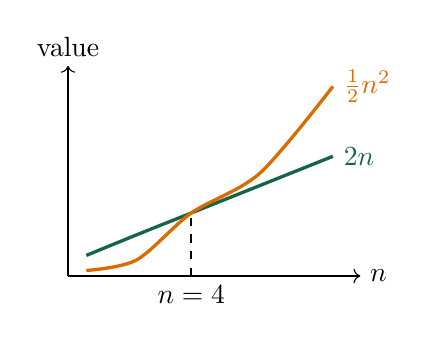
\begin{tikzpicture}[x=0.58cm,y=0.58cm]
          \draw[->] (0,0) -- (6.4,0) node[right] {$n$};
          \draw[->] (0,0) -- (0,4.6) node[above] {value};
          \draw[very thick,ForestGreen]
            plot[smooth] coordinates {(0.4,0.45) (1.5,0.9) (2.7,1.38) (4.2,1.98) (5.8,2.62)}
            node[right] {$2n$};
          \draw[very thick,orange!85!black]
            plot[smooth] coordinates {(0.4,0.12) (1.5,0.35) (2.7,1.38) (4.2,2.25) (5.8,4.15)}
            node[right] {$\frac12 n^2$};
          \draw[dashed,thick] (2.7,0) -- (2.7,1.38);
          \node[below] at (2.7,0) {$n=4$};
        \end{tikzpicture}

        {\scriptsize after the crossing, quadratic growth dominates}
      \end{center}
    \end{column}
  \end{columns}
\end{frame}














\begin{frame}{Comparing two functions on $\mathbb{N}$}
  \begin{block}{Can you give more examples of function $f(n)$ such that $f(n)<\frac{1}{2}n^2$?}
   Determine \textbf{one possible} $n_0\in \mathbb{N}$ such that
   \begin{itemize}
       %\item $f(n)=n^3-2$
       %\item $f(n)=15n^2+5n+80$
       \item $f(n)=n\log n < \frac{1}{2}n^2$ for $n> n_0$
       \item $f(n)=n+1< \frac{1}{2}n^2$ for $n> n_0$
       \item $f(n)=\sqrt{n}< \frac{1}{2}n^2$ for $n> n_0$
       \item $f(n)=\log n< \frac{1}{2}n^2$ for $n> n_0$
       %\item $f(n)=n^a$, for any $a\le 1$
       \item $f(n)=3< \frac{1}{2}n^2$ for $n> n_0$
   \end{itemize}
   {\small \textbf{Note:} Many choices may work. Any valid threshold is acceptable; it does not have to be the smallest.}
  \end{block}
\end{frame}


\begin{frame}{More examples of function comparison}
  \small
  \begin{columns}[T]
    \begin{column}{0.48\textwidth}
      \begin{block}{$n\log n$ versus $n\sqrt{n}$}
        \centering\scriptsize
        \begin{tabular}{c|r|r}
          \toprule
          $n$ & $n\log n$ & $n\sqrt{n}$ \\
          \midrule
          $16$ & $64$ & $64$ \\
          $64$ & $384$ & $512$ \\
          $256$ & $2{,}048$ & $4{,}096$ \\
          \bottomrule
        \end{tabular}
      \end{block}
      \begin{exampleblock}{Question?}
       Can you prove that, for $n>16$
        \[
          n\log n < n\sqrt n?
        \]
      \end{exampleblock}
    \end{column}
    \begin{column}{0.48\textwidth}
      \begin{block}{$2^n$ versus $n!$}
        \centering\scriptsize
        \begin{tabular}{c|r|r}
          \toprule
          $n$ & $2^n$ & $n!$ \\
          \midrule
          $4$ & $16$ & $24$ \\
          $8$ & $256$ & $40{,}320$ \\
          $12$ & $4{,}096$ & $479{,}001{,}600$ \\
          \bottomrule
        \end{tabular}
      \end{block}
      \begin{alertblock}{Question?}
        Can you prove that, for $n \ge 4$:
        \[
          2^n < n!?
        \]
      \end{alertblock}
    \end{column}
  \end{columns}
  
\end{frame}




\begin{frame}{Big $O$-Notation: upper bound}
  \small
  \begin{block}{Definition}
    For a given function $g(n)$,
    \[
      O(g(n))=\{f(n): \exists c>0,\exists n_0\text{ such that }
      0\le f(n)\le c\,g(n),\ \forall n\ge n_0\}.
    \]
  \end{block}
  {\small\color{red!75!black}\textbf{Important:} $O(g(n))$ is a \textbf{set/class of functions}, not one function. The pair $(c,n_0)$ can be \textbf{any valid pair}; it need not be smallest in any metric.}\vspace{-0.35em}
  \begin{columns}[T]
    \begin{column}{0.46\textwidth}
      \begin{exampleblock}{Interpretation}
        $O(g(n))$ is the class of functions that are eventually \textbf{not larger than}
        a constant multiple of $g(n)$.
      \end{exampleblock}
      \begin{alertblock}{Examples}
        \scriptsize
        \begin{itemize}\setlength{\itemsep}{0.1em}
          \item $2n^2+4n+1\in O(n^2)$
          \item $n\log n,n+1,\sqrt n,\log n,3\in O(n^2)$
          \item $n^3,2^n\notin O(n^2)$
        \end{itemize}
      \end{alertblock}
    \end{column}
    \begin{column}{0.52\textwidth}
      \begin{center}
        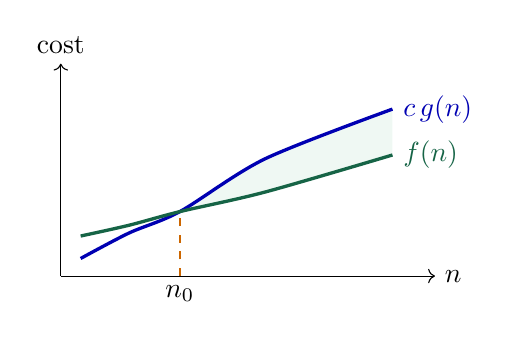
\begin{tikzpicture}[x=0.72cm,y=0.62cm]
          \draw[->] (0,0) -- (6.6,0) node[right] {$n$};
          \draw[->] (0,0) -- (0,4.35) node[above] {cost};
          \fill[SoftGreen,opacity=0.60]
            (2.10,1.32) -- (3.60,1.72) -- (5.85,2.48) --
            (5.85,3.42) -- (3.60,2.40) -- (2.10,1.32) -- cycle;
          \draw[very thick,blue!70!black]
            plot[smooth] coordinates {(0.35,0.36) (1.20,0.88) (2.10,1.32) (3.60,2.40) (5.85,3.42)}
            node[right] {$c\,g(n)$};
          \draw[very thick,ForestGreen]
            plot[smooth] coordinates {(0.35,0.82) (1.20,1.04) (2.10,1.32) (3.60,1.72) (5.85,2.48)}
            node[right] {$f(n)$};
          \draw[dashed,thick,orange!80!black] (2.10,0) -- (2.10,1.32);
          \node[below] at (2.10,0) {$n_0$};
        \end{tikzpicture}
      \end{center}
    \end{column}
  \end{columns}
\end{frame}

\begin{frame}{Algorithmic Intuition of Big-$O$ ($\le$ Upper Bound)}
  \begin{alertblock}{What does $f(n) = \mathcal{O}(g(n))$ mean for Algorithms?}
    \small
    \textbf{An algorithm with growth $f(n)$ will \textcolor{ForestGreen}{run no slower} (grow no faster) than $g(n) \times c$ when $n$ is sufficiently large.}
    \begin{itemize}
      \item $f(n)$ is \textbf{capped from above} by $c \cdot g(n)$ for all $n \ge n_0$.
      \item Represents a \textbf{worst-case upper bound} (guarantees execution time ceiling).
    \end{itemize}
  \end{alertblock}
  \vspace{0.2em}
  \begin{columns}[T]
    \begin{column}{0.49\textwidth}
      \begin{block}{Fast Growth Classes ($\le$ Linear)}
        \scriptsize
        \begin{itemize}\setlength{\itemsep}{0.2em}
          \item $\mathcal{O}(1)$: Indexing \texttt{A[i]}, Stack \texttt{push/pop}
          \item $\mathcal{O}(\log n)$: \textbf{Binary Search}, Euclid GCD
          \item $\mathcal{O}(n)$: \textbf{Linear Search}, find Max/Min
        \end{itemize}
      \end{block}
    \end{column}
    \begin{column}{0.49\textwidth}
      \begin{block}{Higher Growth Classes}
        \scriptsize
        \begin{itemize}\setlength{\itemsep}{0.2em}
          \item $\mathcal{O}(n\log n)$: \textbf{Merge Sort}, \textbf{Heap Sort}, \textbf{Quick Sort}
          \item $\mathcal{O}(n^2)$: \textbf{Bubble Sort}, \textbf{Selection Sort}
          \item $\mathcal{O}(2^n)$: Naive Recursive Fibonacci, TSP
        \end{itemize}
      \end{block}
    \end{column}
  \end{columns}
\end{frame}

\begin{frame}{Quick check: Big $O$}
  \small
  \begin{block}{Exercise}
    For each statement, decide whether it is true or false. If true, give possible constants
    $c$ and $n_0$. If false, explain which term grows too fast.
  \end{block}
  \begin{center}
    \renewcommand{\arraystretch}{1.22}
    \begin{tabular}{c|L{0.62\textwidth}|c}
      \toprule
      & \textbf{Statement} & \textbf{True/False} \\
      \midrule
      1 & $4n+20\in O(n)$ & \\ \addlinespace
      2 & $3n^2+10n+7\in O(n^2)$ & \\ \addlinespace
      3 & $n^2+100n\in O(n)$ & \\ \addlinespace
      4 & $n\log_2 n+50n\in O(n\log n)$ & \\ \addlinespace
      5 & $2^n\in O(n^3)$ & \\
      \bottomrule
    \end{tabular}
  \end{center}
\end{frame}


\begin{frame}{Big $O$-notation Properties}
  \small
  \begin{block}{Properties}
       \begin{itemize}
            \item $O(c\cdot f(n))=O(f(n))$ for any constant $c>0$.
              \begin{itemize}
                \item[] \emph{Example:} $O(4n^2)=O(\frac{1}{4}n^2)=O(n^2)$.
              \end{itemize}
            \item If $f(n) \in O(g(n))$ and $h(n) \in O(k(n))$, then
            $f(n) + h(n)\in O(\max\{g(n), k(n)\})$.
              \begin{itemize}
                \item[] \emph{Example:} if $f(n) \in O(n^2)$ and $h(n) \in O(n^3)$, then
                $f(n) + h(n) \in O(\max\{n^2,n^3\}) = O(n^3)$.
              \end{itemize}
            \item If $f(n) \in O(g(n))$ and $h(n) \in O(k(n))$, then
            $f(n)\cdot h(n) \in O(g(n)\cdot k(n))$.
              \begin{itemize}
                \item[] \emph{Example:} if $f(n) \in O(n^2)$ and $h(n) \in O(n^3)$, then
                $f(n)\cdot h(n) \in O(n^5)$.
              \end{itemize}
        \end{itemize}
      \end{block}
\end{frame}


\begin{frame}{Big $O$-Notation}
  \begin{block}{Example}
  Prove that:
  \[
  O(5n^3+4n^2+5n+7) = O(n^3)
  \]
\end{block}\pause

 \begin{alertblock}{Note}
        For every polynomial of degree $p\ge 1$ with leading coefficient $a_p>0$:
        \[
  O(a_p n^p + a_{p-1} n^{p-1} + \cdots + a_1n +a_0) = O(n^p)
  \]
      \end{alertblock}
\end{frame}







\begin{frame}{Big $\Omega$-Notation: lower bound}
  \small
  \begin{block}{Definition}
    For a given function $g(n)$,
    \[
      \Omega(g(n))=\{f(n): \exists c>0,\exists n_0\text{ such that }
      0\le c\,g(n)\le f(n),\ \forall n\ge n_0\}.
    \]
  \end{block}
  {\small\color{red!75!black}\textbf{Important:} $\Omega(g(n))$ is a \textbf{set/class of functions}, not one function. The pair $(c,n_0)$ can be \textbf{any valid pair}; it need not be smallest in any metric.}\vspace{-0.35em}
  \begin{columns}[T]
    \begin{column}{0.46\textwidth}
      \begin{exampleblock}{Interpretation}
        $\Omega(g(n))$ is the class of functions that are eventually
        \textbf{at least as large as} a constant multiple of $g(n)$.
      \end{exampleblock}
      \begin{alertblock}{Examples}
        \scriptsize
        \begin{itemize}\setlength{\itemsep}{0.1em}
          \item $2^n,n^2,n\log n,n+1\in \Omega(n)$
          \item $\frac12 n-1\in \Omega(n)$
          \item $\sqrt n,\log n,3\notin \Omega(n)$
        \end{itemize}
      \end{alertblock}
    \end{column}
    \begin{column}{0.52\textwidth}
      \begin{center}
        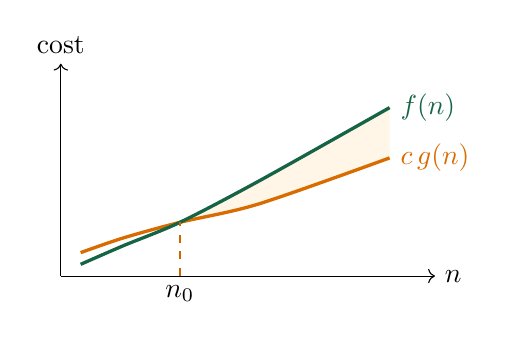
\begin{tikzpicture}[x=0.72cm,y=0.62cm]
          \draw[->] (0,0) -- (6.6,0) node[right] {$n$};
          \draw[->] (0,0) -- (0,4.35) node[above] {cost};
          \fill[SoftOrange,opacity=0.66]
            (2.10,1.10) -- (3.50,1.95) -- (5.80,3.45) --
            (5.80,2.42) -- (3.50,1.48) -- (2.10,1.10) -- cycle;
          \draw[very thick,orange!85!black]
            plot[smooth] coordinates {(0.35,0.48) (1.10,0.78) (2.10,1.10) (3.50,1.48) (5.80,2.42)}
            node[right] {$c\,g(n)$};
          \draw[very thick,ForestGreen]
            plot[smooth] coordinates {(0.35,0.24) (1.10,0.62) (2.10,1.10) (3.50,1.95) (5.80,3.45)}
            node[right] {$f(n)$};
          \draw[dashed,thick,orange!80!black] (2.10,0) -- (2.10,1.10);
          \node[below] at (2.10,0) {$n_0$};
        \end{tikzpicture}
      \end{center}
    \end{column}
  \end{columns}
\end{frame}

\begin{frame}{Algorithmic Intuition of Big-$\Omega$ ($\ge$ Lower Bound)}
  \begin{alertblock}{What does $f(n) = \Omega(g(n))$ mean for Algorithms?}
    \small
    \textbf{An algorithm with growth $f(n)$ will \textcolor{ForestGreen}{take at least} $g(n) \times c$ operations when $n$ is sufficiently large (cannot run faster than this bound).}
    \begin{itemize}
      \item $f(n)$ is \textbf{bounded from below} by $c \cdot g(n)$ for all $n \ge n_0$.
      \item Proves the \textbf{minimum computational effort} required by an algorithm or problem.
    \end{itemize}
  \end{alertblock}
  \vspace{0.2em}
  \begin{columns}[T]
    \begin{column}{0.49\textwidth}
      \begin{block}{Algorithm Lower Bounds}
        \scriptsize
        \begin{itemize}\setlength{\itemsep}{0.2em}
          \item $\Omega(1)$: Best case of Linear Search
          \item $\Omega(n)$: Best case of Insertion Sort
          \item $\Omega(n^2)$: Worst case of Bubble Sort
        \end{itemize}
      \end{block}
    \end{column}
    \begin{column}{0.49\textwidth}
      \begin{block}{Problem Lower Bounds}
        \scriptsize
        \begin{itemize}\setlength{\itemsep}{0.2em}
          \item Finding Min in unsorted array is $\Omega(n)$
          \item Comparison-based Sorting is $\Omega(n\log n)$
          \item Matrix multiplication is $\Omega(n^2)$
        \end{itemize}
      \end{block}
    \end{column}
  \end{columns}
\end{frame}

\begin{frame}{Quick check: Big $\Omega$}
  \small
  \begin{block}{Exercise}
    For each statement, decide whether it is true or false. Focus on whether the left-hand
    function eventually grows at least as fast as the right-hand growth class.
  \end{block}
  \begin{center}
    \renewcommand{\arraystretch}{1.22}
    \begin{tabular}{c|L{0.62\textwidth}|c}
      \toprule
      & \textbf{Statement} & \textbf{True/False} \\
      \midrule
      1 & $7n+3\in \Omega(n)$ & \\ \addlinespace
      2 & $n^2+5n\in \Omega(n^2)$ & \\ \addlinespace
      3 & $\log n\in \Omega(n)$ & \\ \addlinespace
      4 & $2^n\in \Omega(n^3)$ & \\ \addlinespace
      5 & $n\log n\in \Omega(n^2)$ & \\
      \bottomrule
    \end{tabular}
  \end{center}
\end{frame}






\begin{frame}{Big $\Theta$-Notation: tight bound}
  \small
  \begin{block}{Definition}
    For a given function $g(n)$,
    \[
      \Theta(g(n))=\{f(n): \exists c_1,c_2>0,\exists n_0\text{ such that }
      0\le c_1g(n)\le f(n)\le c_2g(n),\ \forall n\ge n_0\}.
    \]
  \end{block}
  {\small\color{red!75!black}\textbf{Important:} $\Theta(g(n))$ is a \textbf{set/class of functions}, not one function. The triple $(c_1,c_2,n_0)$ can be \textbf{any valid choice}; it need not be smallest in any metric.}\vspace{-0.35em}
  \begin{columns}[T]
    \begin{column}{0.43\textwidth}
      \begin{exampleblock}{Interpretation}
        $\Theta(g(n))$ means $f(n)$ is eventually squeezed between two constant
        multiples of $g(n)$. It is a \textbf{tight} growth bound.
      \end{exampleblock}
      \begin{alertblock}{Examples}
        \scriptsize
        \begin{itemize}\setlength{\itemsep}{0.1em}
          \item $n+1,2n-1,\frac12 n+3\in \Theta(n)$
          \item $n^2,\sqrt n,\log n,3\notin \Theta(n)$
        \end{itemize}
      \end{alertblock}
    \end{column}
    \begin{column}{0.55\textwidth}
      \begin{center}
        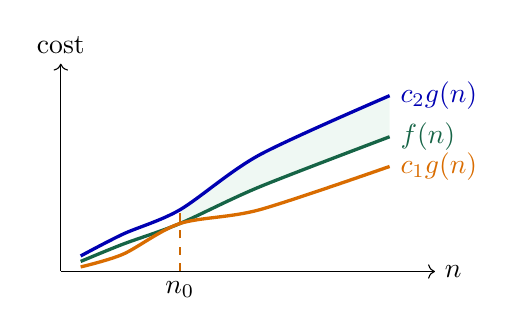
\begin{tikzpicture}[x=0.72cm,y=0.58cm]
          \draw[->] (0,0) -- (6.6,0) node[right] {$n$};
          \draw[->] (0,0) -- (0,4.55) node[above] {cost};
          \fill[SoftGreen,opacity=0.60]
            (2.10,1.05) -- (3.50,1.85) -- (5.80,2.95) --
            (5.80,3.85) -- (3.50,2.55) -- (2.10,1.35) -- cycle;
          \draw[very thick,blue!70!black]
            plot[smooth] coordinates {(0.35,0.34) (1.10,0.82) (2.10,1.35) (3.50,2.55) (5.80,3.85)}
            node[right] {$c_2g(n)$};
          \draw[very thick,ForestGreen]
            plot[smooth] coordinates {(0.35,0.22) (1.10,0.60) (2.10,1.05) (3.50,1.85) (5.80,2.95)}
            node[right] {$f(n)$};
          \draw[very thick,orange!85!black]
            plot[smooth] coordinates {(0.35,0.10) (1.10,0.38) (2.10,1.05) (3.50,1.35) (5.80,2.30)}
            node[right] {$c_1g(n)$};
          \draw[dashed,thick,orange!80!black] (2.10,0) -- (2.10,1.35);
          \node[below] at (2.10,0) {$n_0$};
        \end{tikzpicture}
      \end{center}
    \end{column}
  \end{columns}
\end{frame}

\begin{frame}{Algorithmic Intuition of Big-$\Theta$ ($=$ Tight Bound)}
  \begin{alertblock}{What does $f(n) = \Theta(g(n))$ mean for Algorithms?}
    \small
    \textbf{An algorithm with growth $f(n)$ will \textcolor{ForestGreen}{grow at the exact same rate} as $g(n)$ when $n$ is sufficiently large.}
    \begin{itemize}
      \item $f(n)$ is \textbf{tightly sandwiched}: $c_1 g(n) \le f(n) \le c_2 g(n)$ for all $n \ge n_0$.
      \item Holds if and only if $f(n) \in \mathcal{O}(g(n))$ AND $f(n) \in \Omega(g(n))$.
    \end{itemize}
  \end{alertblock}
  \vspace{0.2em}
  \begin{columns}[T]
    \begin{column}{0.49\textwidth}
      \begin{block}{Algorithm Tight Bounds ($\Theta$)}
        \scriptsize
        \begin{itemize}\setlength{\itemsep}{0.2em}
          \item $\Theta(1)$: Python \texttt{len(list)}, \texttt{A[i]}
          \item $\Theta(n)$: Linear Search (worst case)
          \item $\Theta(n\log n)$: \textbf{Merge Sort} (all cases)
        \end{itemize}
      \end{block}
    \end{column}
    \begin{column}{0.49\textwidth}
      \begin{block}{Quadratic / Cubic Bounds ($\Theta$)}
        \scriptsize
        \begin{itemize}\setlength{\itemsep}{0.2em}
          \item $\Theta(n^2)$: \textbf{Selection Sort} (all cases)
          \item $\Theta(n^2)$: Insertion Sort (worst case)
          \item $\Theta(n^3)$: Floyd-Warshall shortest paths
        \end{itemize}
      \end{block}
    \end{column}
  \end{columns}
\end{frame}

\begin{frame}{Quick check: Big $\Theta$}
  \small
  \begin{block}{Exercise}
    For each running-time function, decide whether it is $\Theta(g(n))$ for the given
    growth class. Explain using both an upper and a lower bound.
  \end{block}
  \begin{center}
    \renewcommand{\arraystretch}{1.22}
    \begin{tabular}{c|L{0.48\textwidth}|c|c}
      \toprule
      & \textbf{Function $f(n)$} & \textbf{Claim} & \textbf{True/False} \\
      \midrule
      1 & $5n+8$ & $\Theta(n)$ & \\ \addlinespace
      2 & $3n^2+n\log n$ & $\Theta(n^2)$ & \\ \addlinespace
      3 & $n^2+100n$ & $\Theta(n)$ & \\ \addlinespace
      4 & $7\log n+2$ & $\Theta(\log n)$ & \\ \addlinespace
      5 & $2^n+n^{10}$ & $\Theta(n^{10})$ & \\
      \bottomrule
    \end{tabular}
  \end{center}
\end{frame}


\begin{frame}{Properties of Big $\Theta$ and $\Omega$ Notations}
  \begin{block}{Properties}
       \begin{itemize}
            \item $\Omega(c\cdot f(n))=\Omega(f(n))$ for any constant $c>0$
            \item If $f(n) \in \Omega(g(n))$ and $h(n) \in \Omega(k(n))$, then $f(n) + h(n)\in \Omega(\max\{g(n), k(n)\})$ 
            \item If $f(n) \in \Omega(g(n))$ and $h(n) \in \Omega(k(n))$, then $f(n)\cdot h(n) \in \Omega(g(n)\cdot k(n))$.
        \end{itemize}
    These properties also hold for $\Theta$ notation.    
      \end{block}
\end{frame}


\begin{frame}{Common function classes}
  \small
  \begin{center}
    \begin{tabular}{cccccc}
      \toprule
      $1$ & $\log n$ & $n$ & $n\log n$ & $n^2$ & $2^n$ \\
      \midrule
      constant & logarithmic & linear & quasi-linear & quadratic & exponential \\
      \bottomrule
    \end{tabular}
  \end{center}
  \vspace{0em}
  \begin{center}
    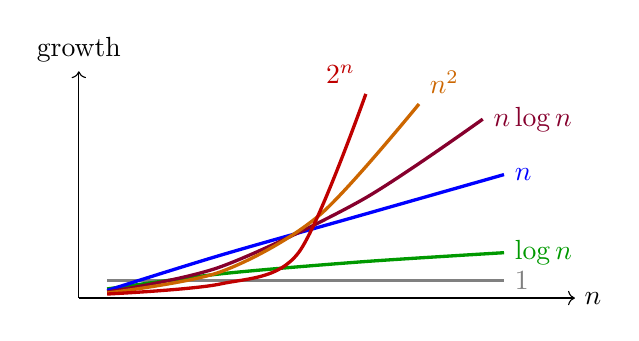
\begin{tikzpicture}[x=0.9cm,y=0.64cm]
      \draw[->] (0,0) -- (7.0,0) node[right] {$n$};
      \draw[->] (0,0) -- (0,4.5) node[above] {growth};
      \draw[very thick,gray]
        plot coordinates {(0.4,0.35) (6.0,0.35)}
        node[right] {$1$};
      \draw[very thick,green!60!black]
        plot[smooth] coordinates {(0.4,0.18) (2.0,0.48) (4.0,0.72) (6.0,0.9)}
        node[right] {$\log n$};
      \draw[very thick,blue]
        plot[smooth] coordinates {(0.4,0.15) (2.0,0.85) (4.0,1.65) (6.0,2.45)}
        node[right] {$n$};
      \draw[very thick,purple!70!black]
        plot[smooth] coordinates {(0.4,0.12) (2.0,0.62) (4.0,1.95) (5.7,3.55)}
        node[right] {$n\log n$};
      \draw[very thick,orange!80!black]
        plot[smooth] coordinates {(0.4,0.1) (2.0,0.52) (3.4,1.65) (4.8,3.85)}
        node[above right] {$n^2$};
      \draw[very thick,red!75!black]
        plot[smooth] coordinates {(0.4,0.08) (2.0,0.28) (3.1,0.9) (4.05,4.05)}
        node[above left] {$2^n$};
    \end{tikzpicture}
  \end{center}
\end{frame}

\begin{frame}{Intuitive Meaning of $\mathcal{O}$, $\Omega$, and $\Theta$ at a Glance}
  \begin{columns}[T]
    \begin{column}{0.32\textwidth}
      \begin{tcolorbox}[colframe=blue!70!black,colback=SoftBlue!35,title={\centering\bfseries $\mathcal{O}(g(n))$: Upper Bound},arc=1.5mm]
        \scriptsize
        \textbf{Analogy:} $\le$ (\textit{No slower than})
        \vspace{0.3em}
        
        $f(n) \le c \cdot g(n)$
        \vspace{0.3em}
        
        \textbf{Meaning:} Cost grows \textbf{at most as fast as} $c \cdot g(n)$ as $n \to \infty$.
        \vspace{0.3em}
        
        \textit{Guarantees worst-case ceiling.}
      \end{tcolorbox}
    \end{column}
    \begin{column}{0.32\textwidth}
      \begin{tcolorbox}[colframe=orange!85!black,colback=SoftOrange!35,title={\centering\bfseries $\Omega(g(n))$: Lower Bound},arc=1.5mm]
        \scriptsize
        \textbf{Analogy:} $\ge$ (\textit{At least as slow as})
        \vspace{0.3em}
        
        $f(n) \ge c \cdot g(n)$
        \vspace{0.3em}
        
        \textbf{Meaning:} Cost is \textbf{at least} $c \cdot g(n)$ for large $n$.
        \vspace{0.3em}
        
        \textit{Proves problem hardness / baseline.}
      \end{tcolorbox}
    \end{column}
    \begin{column}{0.32\textwidth}
      \begin{tcolorbox}[colframe=ForestGreen,colback=SoftGreen!35,title={\centering\bfseries $\Theta(g(n))$: Tight Bound},arc=1.5mm]
        \scriptsize
        \textbf{Analogy:} $\approx$ (\textit{Same rate as})
        \vspace{0.3em}
        
        $c_1 g(n) \le f(n) \le c_2 g(n)$
        \vspace{0.3em}
        
        \textbf{Meaning:} Cost grows at the \textbf{exact same rate}.
        \vspace{0.3em}
        
        \textit{Both $\mathcal{O}(g(n))$ and $\Omega(g(n))$ hold.}
      \end{tcolorbox}
    \end{column}
  \end{columns}
  \vspace{0.3em}
  \begin{alertblock}{Summary for Programmers}
    \centering\scriptsize
    \textbf{Saying $f(n) = \mathcal{O}(g(n))$ means:} For large input size $n$, the algorithm with cost $f(n)$ will \textbf{never run slower} than $g(n) \times \text{constant}$.
  \end{alertblock}
\end{frame}

\begin{frame}{Classic Named Algorithms by Complexity Class}
  \centering\scriptsize
  \renewcommand{\arraystretch}{1.16}
  \begin{tabular}{l l p{4.6cm} p{3.4cm}}
    \toprule
    \textbf{Class} & \textbf{Name} & \textbf{Representative Algorithms / Operations} & \textbf{Practical Scalability} \\
    \midrule
    $\mathcal{O}(1)$ & Constant & Array index \texttt{A[i]}, Stack \texttt{push/pop}, Hash map & Instantaneous ($< 1$ $\mu$s) \\
    $\mathcal{O}(\log n)$ & Logarithmic & \textbf{Binary Search}, Balanced BST lookup, Euclid GCD & Ultra fast ($n=10^9 \implies 30$ ops) \\
    $\mathcal{O}(n)$ & Linear & \textbf{Linear Search}, find Max/Min, List traversal & Scales proportionally with $n$ \\
    $\mathcal{O}(n\log n)$ & Quasi-linear & \textbf{Merge Sort}, \textbf{Heap Sort}, \textbf{Quick Sort} (avg) & Optimal for general sorting \\
    $\mathcal{O}(n^2)$ & Quadratic & \textbf{Bubble Sort}, \textbf{Selection Sort}, \textbf{Insertion Sort} & Feasible for $n \le 10^4$ \\
    $\mathcal{O}(n^3)$ & Cubic & Matrix Multiplication, \textbf{Floyd-Warshall} & Feasible for $n \le 10^3$ \\
    $\mathcal{O}(2^n)$ & Exponential & Naive Fibonacci, Subset Sum (brute force) & Impractical for $n > 40$ \\
    $\mathcal{O}(n!)$ & Factorial & Generating permutations, \textbf{TSP} (brute force) & Impractical for $n > 12$ \\
    \bottomrule
  \end{tabular}
\end{frame}

\begin{frame}{Understanding $\Omega$ and $\Theta$ with Real Algorithm Examples}
  \begin{columns}[T]
    \begin{column}{0.49\textwidth}
      \begin{block}{Lower Bound $\Omega$ Examples}
        \scriptsize
        \begin{itemize}\setlength{\itemsep}{0.25em}
          \item \textbf{Finding Minimum is $\Omega(n)$:}
            Must inspect every element in an unsorted array $\implies$ no algorithm can beat $\Omega(n)$.
          \item \textbf{Comparison Sorting is $\Omega(n\log n)$:}
            Any comparison sort (MergeSort, QuickSort) must make $\ge \Omega(n\log n)$ comparisons in the worst case.
          \item \textbf{Adjacent-Swap Sorts are $\Omega(n^2)$:}
            Any sort swapping only adjacent elements requires $\Omega(n^2)$ in the worst case.
        \end{itemize}
      \end{block}
    \end{column}
    \begin{column}{0.49\textwidth}
      \begin{exampleblock}{Tight Bound $\Theta$ Examples}
        \scriptsize
        \begin{itemize}\setlength{\itemsep}{0.25em}
          \item \textbf{Merge Sort is $\Theta(n\log n)$:}
            Always splits in half and merges $\implies \Theta(n\log n)$ in \textbf{Best, Worst, and Average} cases!
          \item \textbf{Selection Sort is $\Theta(n^2)$:}
            Always scans the rest of the array $\implies \Theta(n^2)$ in \textbf{all cases}, even if already sorted.
          \item \textbf{Linear Search (Worst-Case) is $\Theta(n)$:}
            Traversing all $n$ elements takes exact linear time.
          \item \textbf{Python \texttt{len(list)} is $\Theta(1)$:}
            Stored as a struct field, always constant time.
        \end{itemize}
      \end{exampleblock}
    \end{column}
  \end{columns}
\end{frame}









\begin{frame}{Example}
  %\scriptsize
  \begin{block}{Question}
    For each function, identify the dominant term, remove its
    constant coefficient, and write the simplest Big-$O$ bound.
  \end{block}
  \begin{center}
    \renewcommand{\arraystretch}{1.12}
    \begin{tabular}{c|c|c}
      \toprule
      & \textbf{Running-time function} & \textbf{Big-$O$} \\
      \midrule
      1 & $T(n)=25$ & \rule{2.2cm}{0.4pt} \\
      2 & $T(n)=8n+40$ & \rule{2.2cm}{0.4pt} \\
      3 & $T(n)=5n\log_2 n+2n$ & \rule{2.2cm}{0.4pt} \\
      4 & $T(n)=12n^2+3n+7$ & \rule{2.2cm}{0.4pt} \\
      5 & $T(n)=n^3+50n^2+10n$ & \rule{2.2cm}{0.4pt} \\
      6 & $T(n)=n^2+n\log_2 n+1000$ & \rule{2.2cm}{0.4pt} \\
      \bottomrule
    \end{tabular}
  \end{center}
\end{frame}


\begin{frame}{More practice: simplify $T(n)$}
  \small
  \begin{block}{Question}
    For each function, identify the dominant growth term and write the
    simplest Big-$O$ bound. Assume $n\ge2$.
  \end{block}
  \begin{center}
    \renewcommand{\arraystretch}{1.18}
    \begin{tabular}{c|c|c}
      \toprule
      & \textbf{Running-time function} & \textbf{Big-$O$} \\
      \midrule
      1 & $T(n)=18\log_2 n+7$ & \rule{2.2cm}{0.4pt} \\
      2 & $T(n)=9n\sqrt n+4n$ & \rule{2.2cm}{0.4pt} \\
      3 & $T(n)=\displaystyle\sum_{i=1}^{n}(3i+2)$ & \rule{2.2cm}{0.4pt} \\
      4 & $T(n)=2n^2\log_2 n+6n^2+1$ & \rule{2.2cm}{0.4pt} \\
      5 & $T(n)=5\cdot2^n+n^4$ & \rule{2.2cm}{0.4pt} \\
      6 & $T(n)=n^3+3^n$ & \rule{2.2cm}{0.4pt} \\
      \bottomrule
    \end{tabular}
  \end{center}
\end{frame}













\begin{frame}{How to simplify a running-time function}
  \small
  \begin{block}{Big-$O$ rule}
    Keep the fastest-growing term and ignore constant factors and smaller terms.
  \end{block}
  \vspace{0.25em}
  \begin{center}
    \begin{tabular}{L{0.30\textwidth}L{0.25\textwidth}L{0.29\textwidth}}
      \toprule
      \textbf{Worst-case operation count} & \textbf{Keep} & \textbf{Big-$O$} \\
      \midrule
      $T(n)=7$ & constant & $O(1)$ \\
      \addlinespace
      $T(n)=3n+5$ & $n$ & $O(n)$ \\
      \addlinespace
      $T(n)=2n^2+n$ & $n^2$ & $O(n^2)$ \\
      \bottomrule
    \end{tabular}
  \end{center}
  \vspace{0.4em}
  \begin{exampleblock}{Why ignore constants?}
    For large $n$, $3n+5$ and $n$ grow in the same linear pattern; the factor
    $3$ changes the amount of work, but not the growth class.
  \end{exampleblock}
\end{frame}











% =============================================================
% Example 1: Pair Scoring Algorithm
% =============================================================
\begin{frame}{Pair Scoring Algorithm: Problem \& Core Idea}
  \begin{columns}[T]
    \begin{column}{0.48\textwidth}
      \begin{block}{Problem Definition}
        \scriptsize
        Given an array \texttt{values} of $n$ numbers, compute an aggregated score by performing two independent operations for each element at index $i$:
        \begin{enumerate}\setlength{\itemsep}{0.15em}
          \item Compare with every element to its right.
          \item Accumulate $A[i]$ in geometric doubling steps ($1, 2, 4, \dots$).
        \end{enumerate}
      \end{block}
      \begin{tcolorbox}[colframe=ForestGreen,colback=SoftGreen!30,title={\centering\bfseries Loop Invariant},arc=1.5mm]
        \scriptsize
        After step $i$, \texttt{score} reflects all valid comparisons and log-accumulations for the entire prefix $0 \dots i$.
      \end{tcolorbox}
    \end{column}
    \begin{column}{0.50\textwidth}
      \begin{center}
        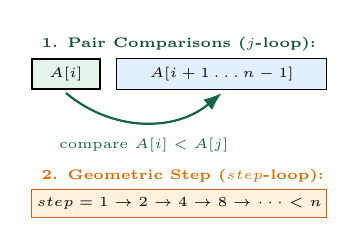
\begin{tikzpicture}[x=0.72cm,y=0.48cm]
          % Step 1: Pair comparisons
          \node[anchor=west,font=\tiny\bfseries\color{ForestGreen!80!black}] at (0,4.6) {1. Pair Comparisons ($j$-loop):};
          \draw[fill=SoftGreen,thick] (0,3.4) rectangle (1.2,4.2) node[pos=0.5]{\tiny $A[i]$};
          \draw[fill=SoftBlue] (1.5,3.4) rectangle (5.2,4.2) node[pos=0.5]{\tiny $A[i+1 \dots n-1]$};
          \draw[-Latex,thick,ForestGreen] (0.6,3.3) to[out=-40,in=-140] node[below=2pt,font=\tiny\color{ForestGreen!90!black}]{compare $A[i] < A[j]$} (3.35,3.3);

          % Step 2: Geometric while loop (pushed down ~1cm)
          \node[anchor=west,font=\tiny\bfseries\color{orange!85!black}] at (0,1.1) {2. Geometric Step ($step$-loop):};
          \draw[fill=SoftOrange,draw=orange!80!black] (0,0.0) rectangle (5.2,0.75) node[pos=0.5]{\tiny $step = 1 \to 2 \to 4 \to 8 \to \dots < n$};
        \end{tikzpicture}
      \end{center}
      \vspace{-0.2em}
      \begin{exampleblock}{Structure Overview}
        \scriptsize
        Two sequential inner loops inside an outer loop of size $n$.
      \end{exampleblock}
    \end{column}
  \end{columns}
\end{frame}

\begin{frame}[fragile]{Activity: Analyze Pair Scoring Algorithm}
  \scriptsize
  \begin{columns}[T]
    \begin{column}{0.54\textwidth}
\begin{lstlisting}[style=pseudonumbered,basicstyle=\ttfamily]
FUNCTION PAIR_SCORE
INPUT: a sequence values of length n
OUTPUT: a numerical score
    score = 0
    FOR i = 0 TO n - 1 DO
        FOR j = i + 1 TO n - 1 DO
            IF values[i] < values[j] THEN
                score = score + 1
        step = 1
        WHILE step < n DO
            score = score + values[i]
            step = 2 * step
    RETURN score
\end{lstlisting}
    \end{column}
    \begin{column}{0.42\textwidth}
      \begin{block}{Student Task}
        \scriptsize
        Assume each basic operation takes $O(1)$ time.
        \begin{enumerate}\setlength{\itemsep}{0.25em}
          \item \textbf{Pair comparisons ($j$-loop):}\\
            How many comparisons occur over all $i$?
          \item \textbf{Geometric while-loop:}\\
            How many iterations run for each $i$?
          \item \textbf{Total operation count $T(n)$:}\\
            Combine the two parts into a single function.
          \item \textbf{Big-$O$ / Big-$\Theta$ bound:}\\
            State and justify the dominant growth class.
        \end{enumerate}
      \end{block}
    \end{column}
  \end{columns}
\end{frame}

% -------------------------------------------------------------
% Problem 1: Insertion Sort
% -------------------------------------------------------------
\begin{frame}{Insertion Sort: Problem \& Core Idea}
  \begin{columns}[T]
    \begin{column}{0.48\textwidth}
      \begin{block}{Problem Definition}
        \scriptsize
        \textbf{Input:} An array $A[0 \dots n-1]$ of $n$ elements.\\
        \textbf{Output:} $A$ sorted in non-decreasing order:
        \[
          A[0] \le A[1] \le \dots \le A[n-1].
        \]
      \end{block}
      \begin{tcolorbox}[colframe=ForestGreen,colback=SoftGreen!30,title={\centering\bfseries Core Idea (Card Player Analogy)},arc=1.5mm]
        \scriptsize
        \begin{itemize}\setlength{\itemsep}{0.15em}
          \item Pick each element \texttt{key = A[j]} one by one ($j = 1 \to n-1$).
          \item Shift all larger elements in the sorted prefix $A[0 \dots j-1]$ one slot to the right.
          \item Insert \texttt{key} into the created empty slot.
        \end{itemize}
      \end{tcolorbox}
    \end{column}
    \begin{column}{0.50\textwidth}
      \begin{center}
        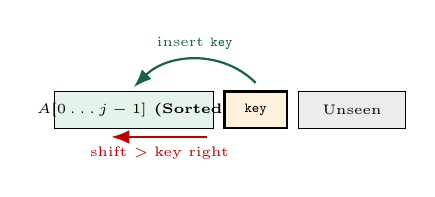
\begin{tikzpicture}[x=0.72cm,y=0.55cm]
          \draw[fill=SoftGreen] (0,0) rectangle (2.8,0.85);
          \node at (1.4,0.42) [font=\tiny\bfseries] {$A[0 \dots j-1]$ (Sorted)};
          \draw[fill=SoftOrange,thick] (3.0,0) rectangle (4.1,0.85);
          \node at (3.55,0.42) [font=\tiny\bfseries] {\texttt{key}};
          \draw[fill=gray!15] (4.3,0) rectangle (6.2,0.85);
          \node at (5.25,0.42) [font=\tiny] {Unseen};
          \draw[-Latex,thick,red!75!black] (2.7,-0.2) -- node[below,font=\tiny]{shift $> \text{key}$ right} (1.0,-0.2);
          \draw[-Latex,thick,ForestGreen] (3.55,1.05) to[out=135,in=45] node[above,font=\tiny]{insert \texttt{key}} (1.4,0.95);
        \end{tikzpicture}
      \end{center}
      \begin{exampleblock}{Loop Invariant}
        \scriptsize
        At the start of step $j$, the subarray $A[0 \dots j-1]$ consists of the elements originally in $A[0 \dots j-1]$, but in \textbf{sorted order}.
      \end{exampleblock}
    \end{column}
  \end{columns}
\end{frame}

\begin{frame}[fragile]{Activity: Analyze Insertion Sort}
  \small
  \begin{columns}[T]
    \begin{column}{0.56\textwidth}
\begin{lstlisting}[style=pseudonumbered,basicstyle=\ttfamily\scriptsize]
FUNCTION INSERTION_SORT(A)
INPUT: array A of length n
OUTPUT: A sorted in non-decreasing order
    FOR j = 1 TO LENGTH(A) - 1 DO
        key = A[j]
        i = j - 1
        WHILE i >= 0 AND A[i] > key DO
            A[i + 1] = A[i]
            i = i - 1
        A[i + 1] = key
    RETURN A
\end{lstlisting}
    \end{column}
    \begin{column}{0.40\textwidth}
      \begin{block}{Student Task}
        \scriptsize
        \begin{enumerate}\setlength{\itemsep}{0.25em}
          \item \textbf{Trace the algorithm:}\\
            Trace on input $[5, 2, 4, 6, 1, 3]$.
          \item \textbf{Best-case scenario (Already sorted):}\\
            Count comparisons and find Big-$O$ bound.
          \item \textbf{Worst-case scenario (Reverse sorted):}\\
            Write summation of shifts and find Big-$O$ bound.
          \item \textbf{Auxiliary space complexity:}\\
            Determine auxiliary space needed.
        \end{enumerate}
      \end{block}
    \end{column}
  \end{columns}
\end{frame}

% -------------------------------------------------------------
% Problem 2: Merge Procedure
% -------------------------------------------------------------
\begin{frame}{Merge Procedure: Problem \& Core Idea}
  \begin{columns}[T]
    \begin{column}{0.48\textwidth}
      \begin{block}{Problem Definition}
        \scriptsize
        \textbf{Input:} Two \textbf{already sorted} arrays $A$ and $B$.\\
        \textbf{Output:} A single sorted array $C$ containing all $n = |A| + |B|$ elements in non-decreasing order.
      \end{block}
      \begin{tcolorbox}[colframe=blue!70!black,colback=SoftBlue!30,title={\centering\bfseries Core Idea (Two-Finger Scan)},arc=1.5mm]
        \scriptsize
        \begin{itemize}\setlength{\itemsep}{0.15em}
          \item Point $i$ at start of $A$, $j$ at start of $B$.
          \item Compare $A[i]$ and $B[j]$.
          \item Append smaller item to $C$ and advance that pointer.
          \item Copy any leftovers when one array is exhausted.
        \end{itemize}
      \end{tcolorbox}
    \end{column}
    \begin{column}{0.50\textwidth}
      \begin{center}
        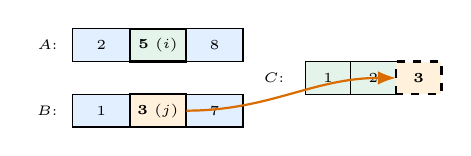
\begin{tikzpicture}[x=0.72cm,y=0.52cm]
          % Array A
          \node[font=\tiny,anchor=east] at (-0.1,2.4) {$A$:};
          \draw[fill=SoftBlue] (0,2) rectangle (1.0,2.8) node[pos=0.5]{\tiny 2};
          \draw[fill=SoftGreen,thick] (1.0,2) rectangle (2.0,2.8) node[pos=0.5]{\tiny \textbf{5} ($i$)};
          \draw[fill=SoftBlue] (2.0,2) rectangle (3.0,2.8) node[pos=0.5]{\tiny 8};
          % Array B
          \node[font=\tiny,anchor=east] at (-0.1,0.8) {$B$:};
          \draw[fill=SoftBlue] (0,0.4) rectangle (1.0,1.2) node[pos=0.5]{\tiny 1};
          \draw[fill=SoftOrange,thick] (1.0,0.4) rectangle (2.0,1.2) node[pos=0.5]{\tiny \textbf{3} ($j$)};
          \draw[fill=SoftBlue] (2.0,0.4) rectangle (3.0,1.2) node[pos=0.5]{\tiny 7};
          % Array C
          \node[font=\tiny,anchor=east] at (3.9,1.6) {$C$:};
          \draw[fill=SoftGreen] (4.1,1.2) rectangle (4.9,2.0) node[pos=0.5]{\tiny 1};
          \draw[fill=SoftGreen] (4.9,1.2) rectangle (5.7,2.0) node[pos=0.5]{\tiny 2};
          \draw[fill=SoftOrange,dashed,thick] (5.7,1.2) rectangle (6.5,2.0) node[pos=0.5]{\tiny \textbf{3}};
          \draw[-Latex,thick,orange!85!black] (2.0,0.8) to[out=0,in=180] (5.7,1.6);
        \end{tikzpicture}
      \end{center}
      \begin{exampleblock}{Loop Invariant}
        \scriptsize
        $C[0 \dots i+j-1]$ always contains the $i+j$ smallest elements of $A \cup B$ in sorted order.
      \end{exampleblock}
    \end{column}
  \end{columns}
\end{frame}

\begin{frame}[fragile]{Activity: Analyze the Merge Procedure}
  \scriptsize
  \begin{columns}[T]
    \begin{column}{0.57\textwidth}
\begin{lstlisting}[style=pseudonumbered,basicstyle=\ttfamily\scriptsize]
FUNCTION MERGE(A, B)
INPUT: sorted arrays A and B
OUTPUT: sorted array C containing all values
    CREATE an empty array C
    i = 0; j = 0
    WHILE i < LENGTH(A) AND j < LENGTH(B) DO
        IF A[i] <= B[j] THEN
            APPEND A[i] to C; i = i + 1
        ELSE
            APPEND B[j] to C; j = j + 1
    WHILE i < LENGTH(A) DO
        APPEND A[i] to C; i = i + 1
    WHILE j < LENGTH(B) DO
        APPEND B[j] to C; j = j + 1
    RETURN C
\end{lstlisting}
    \end{column}
    \begin{column}{0.39\textwidth}
      \begin{block}{Student Task}
        \scriptsize
        Let $n = |A| + |B|$.
        \begin{enumerate}\setlength{\itemsep}{0.25em}
          \item \textbf{Trace the procedure:}\\
            Trace for $[2, 5, 8]$ and $[1, 3, 7]$.
          \item \textbf{Element comparisons:}\\
            Maximum comparisons \texttt{A[i] <= B[j]}.
          \item \textbf{Append operations:}\\
            Total elements appended into $C$.
          \item \textbf{Time complexity:}\\
            Find $T(n)$ and its Big-$O$ / Big-$\Theta$ bound.
          \item \textbf{Auxiliary space complexity:}\\
            Memory allocated for array $C$.
        \end{enumerate}
      \end{block}
    \end{column}
  \end{columns}
\end{frame}

% -------------------------------------------------------------
% Problem 3: Quicksort Partition (Simplest with Auxiliary Array)
% -------------------------------------------------------------
\begin{frame}{Array Partitioning: Problem \& Core Idea}
  \begin{columns}[T]
    \begin{column}{0.48\textwidth}
      \begin{block}{Problem Definition}
        \scriptsize
        \textbf{Input:} Subarray $A[low \dots high]$ and pivot $p = A[high]$.\\
        \textbf{Output:} Rearrange elements around $p$ so that elements $\le p$ are placed left, and elements $> p$ are placed right.
      \end{block}
      \vspace{-0.2em}
      \begin{tcolorbox}[colframe=purple!70!black,colback=SoftPurple!30,title={\centering\bfseries Simplest Idea: Auxiliary Array},arc=1.5mm]
        \scriptsize
        Fill a helper array \texttt{temp}:
        \begin{itemize}\setlength{\itemsep}{0.08em}
          \item Items $\le p \implies$ place at \texttt{left} ($\to$).
          \item Items $> p \implies$ place at \texttt{right} ($\leftarrow$).
          \item Place $p$ in the middle, then copy back to $A$.
        \end{itemize}
      \end{tcolorbox}
    \end{column}
    \begin{column}{0.50\textwidth}
      \begin{center}
        \vspace{0.2em}
        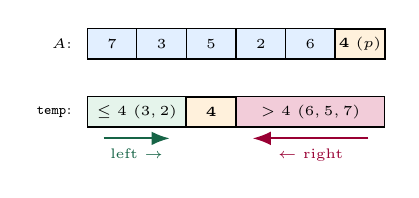
\begin{tikzpicture}[x=0.70cm,y=0.48cm]
          % Original A
          \node[font=\tiny,anchor=east] at (-0.1,2.3) {$A$:};
          \draw[fill=SoftBlue] (0,1.9) rectangle (0.9,2.7) node[pos=0.5]{\tiny 7};
          \draw[fill=SoftBlue] (0.9,1.9) rectangle (1.8,2.7) node[pos=0.5]{\tiny 3};
          \draw[fill=SoftBlue] (1.8,1.9) rectangle (2.7,2.7) node[pos=0.5]{\tiny 5};
          \draw[fill=SoftBlue] (2.7,1.9) rectangle (3.6,2.7) node[pos=0.5]{\tiny 2};
          \draw[fill=SoftBlue] (3.6,1.9) rectangle (4.5,2.7) node[pos=0.5]{\tiny 6};
          \draw[fill=SoftOrange,thick] (4.5,1.9) rectangle (5.4,2.7) node[pos=0.5]{\tiny \textbf{4} ($p$)};
          % Aux temp
          \node[font=\tiny,anchor=east] at (-0.1,0.5) {\texttt{temp}:};
          \draw[fill=SoftGreen] (0,0.1) rectangle (1.8,0.9) node[pos=0.5]{\tiny $\le 4$ ($3, 2$)};
          \draw[fill=SoftOrange,thick] (1.8,0.1) rectangle (2.7,0.9) node[pos=0.5]{\tiny \textbf{4}};
          \draw[fill=purple!20] (2.7,0.1) rectangle (5.4,0.9) node[pos=0.5]{\tiny $> 4$ ($6, 5, 7$)};
          \draw[-Latex,thick,ForestGreen] (0.3,-0.2) -- node[below,font=\tiny]{left $\to$} (1.5,-0.2);
          \draw[-Latex,thick,purple!80!black] (5.1,-0.2) -- node[below,font=\tiny]{$\leftarrow$ right} (3.0,-0.2);
        \end{tikzpicture}
      \end{center}
    \end{column}
  \end{columns}
\end{frame}

\begin{frame}[fragile]{Activity: Analyze Quicksort Partition (Auxiliary Array)}
  \scriptsize
  \begin{columns}[T]
    \begin{column}{0.56\textwidth}
\begin{lstlisting}[style=pseudonumbered,basicstyle=\ttfamily\tiny]
FUNCTION PARTITION_AUX(A, low, high)
INPUT: subarray A[low..high]
OUTPUT: final index of pivot
    pivot = A[high]
    CREATE array temp of size (high - low + 1)
    left = 0
    right = high - low
    FOR i = low TO high - 1 DO
        IF A[i] <= pivot THEN
            temp[left] = A[i]
            left = left + 1
        ELSE
            temp[right] = A[i]
            right = right - 1
    temp[left] = pivot
    COPY temp BACK TO A[low..high]
    RETURN low + left
\end{lstlisting}
    \end{column}
    \begin{column}{0.40\textwidth}
      \begin{block}{Student Task}
        \scriptsize
        Let subarray size $m = high - low + 1$.
        \begin{enumerate}\setlength{\itemsep}{0.25em}
          \item \textbf{Trace the procedure:}\\
            Trace on $[7, 3, 5, 2, 6, 4]$ with pivot $4$.
          \item \textbf{Comparisons with pivot:}\\
            Count comparisons in the \texttt{FOR} loop.
          \item \textbf{Array copy steps:}\\
            Count items moved into and out of \texttt{temp}.
          \item \textbf{Time complexity:}\\
            Find $T(m)$ and its Big-$O$ / Big-$\Theta$ bound.
          \item \textbf{Auxiliary space complexity:}\\
            Memory allocated for array \texttt{temp}.
        \end{enumerate}
      \end{block}
    \end{column}
  \end{columns}
\end{frame}

% =============================================================
\section{Space Complexity}
% =============================================================




\begin{frame}{Space complexity: a practical view}
  \small
  \begin{block}{Definition}
    Space complexity measures the \textbf{maximum memory simultaneously in use}
    during an algorithm. We study how this worst-case requirement grows as the
    input size $n$ grows. Write $S_{\mathrm{total}}(n)$ for total space and
    $S_{\mathrm{aux}}(n)$ for auxiliary space.
  \end{block}
  \begin{center}
    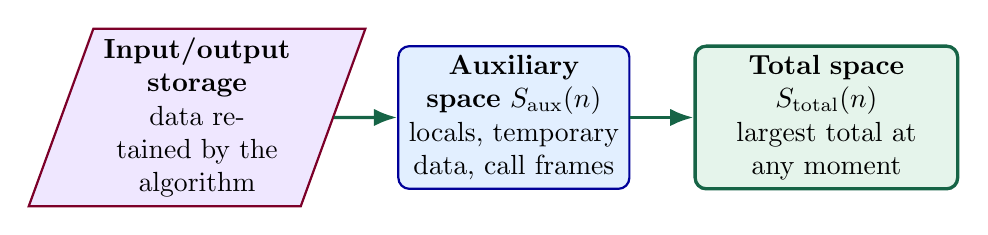
\begin{tikzpicture}[node distance=0.8cm]
      \node[data] (input) {\textbf{Input/output storage}\\data retained by the algorithm};
      \node[process,right=of input] (work) {\textbf{Auxiliary space $S_{\mathrm{aux}}(n)$}\\locals, temporary data, call frames};
      \node[concept,right=of work] (peak) {\textbf{Total space $S_{\mathrm{total}}(n)$}\\largest total at any moment};
      \draw[arrow] (input) -- (work);
      \draw[arrow] (work) -- (peak);
    \end{tikzpicture}
  \end{center}
  \vspace{0.35em}
  \begin{columns}[T]
    \begin{column}{0.48\textwidth}
      \begin{exampleblock}{Total space: $S_{\mathrm{total}}(n)$}
        Counts input, output, and temporary working memory that coexist at the
        peak-memory moment.
      \end{exampleblock}
    \end{column}
    \begin{column}{0.48\textwidth}
      \begin{alertblock}{Auxiliary space: $S_{\mathrm{aux}}(n)$}
        Counts only extra working memory, excluding the input and output. Later
        examples report both measures explicitly.
      \end{alertblock}
    \end{column}
  \end{columns}
\end{frame}

\begin{frame}[fragile]{Examples: calculate $S(n)$}
  \scriptsize
  \begin{block}{Storage model}
    Count one unit for each scalar and each array element. Total space includes
    the input; auxiliary space counts only local working storage.
  \end{block}
  \begin{columns}[T]
    \begin{column}{0.48\textwidth}
      \begin{exampleblock}{Squared distance between two points}
\begin{lstlisting}[style=pseudo,basicstyle=\ttfamily\tiny]
FUNCTION DISTANCE_SQUARED
INPUT: x1, y1, x2, y2
    dx = x2 - x1
    dy = y2 - y1
    answer = dx * dx + dy * dy
    RETURN answer
\end{lstlisting}
        Input: $4$ units. Locals: $3$ units.
        \[
          \begin{aligned}
            S_{\mathrm{total}}(n)&=4+3=7\in\Theta(1),\\
            S_{\mathrm{aux}}(n)&=3\in\Theta(1).
          \end{aligned}
        \]
      \end{exampleblock}
    \end{column}
    \begin{column}{0.48\textwidth}
      \begin{block}{Count positive values}
\begin{lstlisting}[style=pseudo,basicstyle=\ttfamily\tiny]
FUNCTION COUNT_POSITIVE
INPUT: array values of length n
    count = 0
    i = 0
    WHILE i < n DO
        IF values[i] > 0 THEN
            count = count + 1
        i = i + 1
    RETURN count
\end{lstlisting}
        Input: $n$ units. Locals \texttt{count} and \texttt{i}: $2$ units.
        \[
          \begin{aligned}
            S_{\mathrm{total}}(n)&=n+2\in\Theta(n),\\
            S_{\mathrm{aux}}(n)&=2\in\Theta(1).
          \end{aligned}
        \]
      \end{block}
    \end{column}
  \end{columns}
\end{frame}

\begin{frame}[fragile]{Examples: output storage changes $S(n)$}
  \scriptsize
  \begin{block}{Convention}
    Total space includes input and output. Auxiliary space below excludes both
    and counts only loop variables and temporary working data.
  \end{block}
  \begin{columns}[T]
    \begin{column}{0.48\textwidth}
      \begin{exampleblock}{Create a sign mask}
\begin{lstlisting}[style=pseudo,basicstyle=\ttfamily\tiny]
FUNCTION SIGN_MASK
INPUT: array values of length n
OUTPUT: Boolean array mask of length n
    FOR i = 0 TO n - 1 DO
        mask[i] = (values[i] >= 0)
    RETURN mask
\end{lstlisting}
        Input: $n$; output: $n$; index: $1$.
        \[
          \begin{aligned}
            S_{\mathrm{total}}(n)&=2n+1\in\Theta(n),\\
            S_{\mathrm{aux}}(n)&=1\in\Theta(1).
          \end{aligned}
        \]
      \end{exampleblock}
    \end{column}
    \begin{column}{0.48\textwidth}
      \begin{block}{Build a comparison table}
\begin{lstlisting}[style=pseudo,basicstyle=\ttfamily\tiny]
FUNCTION COMPARISON_TABLE
INPUT: array values of length n
OUTPUT: n by n Boolean table
    FOR i = 0 TO n - 1 DO
        FOR j = 0 TO n - 1 DO
            table[i][j] = (values[i] < values[j])
    RETURN table
\end{lstlisting}
        Input: $n$; output: $n^2$; indices: $2$.
        \[
          \begin{aligned}
            S_{\mathrm{total}}(n)&=n^2+n+2\in\Theta(n^2),\\
            S_{\mathrm{aux}}(n)&=2\in\Theta(1).
          \end{aligned}
        \]
      \end{block}
    \end{column}
  \end{columns}
\end{frame}

\begin{frame}[fragile]{Function calls and memory reuse}
  \scriptsize
  \begin{columns}[T]
    \begin{column}{0.50\textwidth}
\begin{lstlisting}[style=pseudo,basicstyle=\ttfamily]
FUNCTION PROCESS_THREE
INPUT: reference to array data of length n
    x = ANALYZE(data)
    y = ANALYZE(data)
    z = ANALYZE(data)
    RETURN x + y + z
    
FUNCTION ANALYZE(data)
INPUT: reference to array data of length n
    temp = a copy of data
    RETURN temp[0]
\end{lstlisting}
      Each call creates one temporary $n$-item array. The input itself is
      shared, because it is passed by reference.
    \end{column}
    \begin{column}{0.46\textwidth}
      \begin{block}{Auxiliary memory over time}
        \centering
        \begin{tabular}{l|c}
          \toprule
          Moment & Memory in use \\
          \midrule
          before call 1 & $c$ \\
          during call 1 & $c+n$ \\
          after call 1 & $c$ \\
          during call 2 & $c+n$ \\
          during call 3 & $c+n$ \\
          \bottomrule
        \end{tabular}
      \end{block}
      \begin{exampleblock}{Peak space}
        Here $c$ is fixed storage retained by \texttt{PROCESS\_THREE}. Only one
        \texttt{temp} exists at a time, so
        \[
          S_{\mathrm{aux}}(n)=n+c\in\Theta(n),
        \]
        not $3n$. A completed call releases its local memory for reuse.
      \end{exampleblock}
    \end{column}
  \end{columns}
\end{frame}


\begin{frame}[fragile]{Example: analyze space usage}
  \scriptsize
  \begin{columns}[T]
    \begin{column}{0.52\textwidth}
\begin{lstlisting}[style=pseudo,basicstyle=\ttfamily]
FUNCTION IS_PALINDROME
INPUT: a bit string bits of length n
OUTPUT: TRUE if the bit string reads the same backward
    reversed = an empty bit string

    FOR i = n - 1 DOWN TO 0 DO
        APPEND bits[i] TO reversed

    FOR i = 0 TO n - 1 DO
        IF bits[i] != reversed[i] THEN
            RETURN FALSE
    RETURN TRUE
\end{lstlisting}
    \end{column}
    \begin{column}{0.44\textwidth}
      \begin{block}{Memory analysis}
        \begin{itemize}
          \item Input string: $n$ bits.
          \item Reversed copy: $n$ additional bits.
          \item Loop index and fixed control data: $O(\log n)$ bits.
        \end{itemize}
      \end{block}
      \begin{exampleblock}{Conclusion}
        The temporary copy dominates, so
        $S_{\mathrm{aux}}(n)\in\Theta(n)$. Total space also satisfies
        $S_{\mathrm{total}}(n)\in\Theta(n)$.
      \end{exampleblock}
      \begin{alertblock}{Can we use less space?}
        Compare matching bits from the two ends without constructing a copy.
        Two indices require $\Theta(\log n)$ bits, or $\Theta(1)$ machine words.
      \end{alertblock}
    \end{column}
  \end{columns}
\end{frame}

\begin{frame}{Key takeaways: algorithms and representations}
  \small
  \begin{itemize}
    \setlength{\itemsep}{0.75em}
    \item \textbf{\color{ForestGreen}Start with the problem:} clearly state the
      accepted inputs and required outputs.
    \item \textbf{\color{ForestGreen}Define the algorithm:} give a finite,
      precise sequence of effective steps that produces the result.
    \item \textbf{\color{ForestGreen}Check all essential properties:} defined
      input/output, definiteness, finiteness, effectiveness, correctness, and
      generality.
    \item \textbf{\color{ForestGreen}Choose a representation:} use a flowchart
      to emphasize control flow or pseudocode to express structured,
      language-neutral steps.
    \item \textbf{\color{ForestGreen}Separate logic from implementation:} one
      algorithm can be implemented as programs in many languages.
    \item \textbf{\color{ForestGreen}Validate systematically:} trace examples
      and edge cases, detect ambiguity or non-termination, and use
      counterexamples to expose incorrectness.
  \end{itemize}
\end{frame}

\begin{frame}{Key takeaways: time and space complexity}
  \small
  \begin{itemize}
    \setlength{\itemsep}{0.25em}
    \item \textbf{\color{ForestGreen}Fix the input size and cost model:}
      describe the problem using $n$ and decide which basic operations count as
      constant-time work.
    \item \textbf{\color{ForestGreen}Build $T(n)$:} add consecutive work,
      account for changing loop bounds, and multiply genuinely nested work.
    \item \textbf{\color{ForestGreen}Recognize common patterns:} full scans are
      linear, nested scans are often quadratic, and repeated doubling or
      halving is logarithmic.
    \item \textbf{\color{ForestGreen}State the case:} best, average, and worst
      cases describe different inputs having the same size.
    \item \textbf{\color{ForestGreen}Classify growth:} $f\in O(g)$ gives an
      upper bound, $f\in\Omega(g)$ a lower bound, and $f\in\Theta(g)$ a tight
      bound; constants and lower-order terms do not determine the class.
    \item \textbf{\color{ForestGreen}Measure peak memory:}
      $S_{\mathrm{total}}(n)$ counts total memory, while
      $S_{\mathrm{aux}}(n)$ counts extra working memory beyond input and output.
  \end{itemize}
\end{frame}

\end{document}
